\documentclass[9pt]{beamer}
\usetheme{Boadilla}

\makeatother
\setbeamertemplate{footline}
{
	\leavevmode%
	\hbox{%
		\begin{beamercolorbox}[wd=.4\paperwidth,ht=2.25ex,dp=1ex,center]{author in head/foot}%
			\usebeamerfont{author in head/foot}\insertshortauthor
		\end{beamercolorbox}%
		\begin{beamercolorbox}[wd=.6\paperwidth,ht=2.25ex,dp=1ex,center]{title in head/foot}%
			\usebeamerfont{title in head/foot}\insertshorttitle\hspace*{3em}
			\insertframenumber{} / \inserttotalframenumber\hspace*{1ex}
	\end{beamercolorbox}}%
	\vskip0pt%
}
\makeatletter
\setbeamertemplate{navigation symbols}{}

\usepackage{tikz}
\usetikzlibrary{positioning}

\usepackage{lipsum}
\usepackage{appendixnumberbeamer}

\usepackage[authoryear]{natbib}
\usepackage[latin1]{inputenc}
\usepackage[T1]{fontenc}
\usepackage{caption}
\usepackage{amsmath, amssymb}
\usepackage{epstopdf}
\usepackage{graphicx}
\usepackage{lmodern}
\usepackage{xcolor}
\usepackage{xpatch}
\usepackage{multirow}

\usepackage{amsmath,theorem,amssymb,graphicx, pgfplots, tabularx, placeins}
\usepackage{dsfont}
\usepackage{caption}
%\usepackage{subcaption}
%\usepackage{subcaption}
\setbeamertemplate{caption}{\raggedright\insertcaption\par}
%\setbeamertemplate{footline}[frame number]
\usepackage{csquotes}
\usepackage{bm}
\bibliographystyle{econometrica}
\usepackage[normalem]{ulem}
\usepackage{booktabs}

\usepackage{setspace}


\definecolor{gray(x11gray)}{rgb}{0.75, 0.75, 0.75}


\newcommand{\bit}{\begin{itemize}}
	\newcommand{\eit}{\end{itemize}}
\newcommand{\ben}{\begin{enumerate}}
	\newcommand{\een}{\end{enumerate}}

\newcommand{\bc}{\color{blue}}
\newcommand{\rc}{\color{red}}


\newcommand{\lb}{\label}
\newcommand{\re}{\eqref}

\title[Course Summary]{Macroeconomics II, Lecture XIV:\\
	Course Summary and Q\&A}
\author{Erik {\"O}berg}
\date{}

\begin{document}

\maketitle

\begin{frame}{This course}
\begin{itemize}
	\setlength\itemsep{1.5em}
	
	\item \textbf{Business-cycle frameworks:} RBC, NK
	\item \textbf{Fricitional labor markets: }McCall, Burdett-Mortensen, DMP
	\item \textbf{Incomplete asset markets: }Consumption-savings dynamics, Aiyagari
\end{itemize}
\end{frame}


\begin{frame}{Today}
\begin{itemize}
	\setlength\itemsep{1.5em}
		
	\item Summarize the course material, by putting these frameworks together in one model: a Heterogenous-Agent New-Keynesian model with Search And Matching frictions --- a \bf HANK \& SAM \normalfont  model
	
	\item Use this ``meta model'' to understand some questions at the research frontier
	
	\item First: some history of >recent< ideas
\end{itemize}
\end{frame}

\begin{frame}{HANK models}
\begin{itemize}
	\setlength\itemsep{1.5em}
	\item \textbf{Heterogeneous Agents New Keynesian} models: NK business cycle
	models with incomplete asset markets (and therefore household heterogeneity)
	\item Why interesting?
	\item Consider the vanilla RANK model:
	\begin{eqnarray*}
		\hat{i}_{t} & = & \phi\pi_{t}+\nu_{t}\\
		\pi_{t} & = & \beta E_{t}\pi_{t+1}+\kappa\hat{y}_{t}\\
		\hat{y}_{t} & = & -(\hat{i}_{t}-E_{t}\pi_{t+1})+E_{t}\hat{y}_{t+1}
	\end{eqnarray*}
	\item What is the transmission mechanism of an MP shock?
\end{itemize}
\end{frame}

\begin{frame}{HANK models}
\begin{itemize}
	\setlength\itemsep{1.5em}
	\item Extended representation of the vanilla RANK model:
	\begin{eqnarray*}
		\hat{i}_{t} & = & \phi\pi_{t}+\nu_{t}\\
		\pi_{t} & = & \beta E_{t}\pi_{t+1}+\kappa\hat{y}_{t}\\
		\hat{c}_{t} & = & -(\hat{i}_{t}-E_{t}\pi_{t+1})+E_{t}\hat{c}_{t+1}\\
		\hat{c_{t}} & = & \hat{y_{t}}
	\end{eqnarray*}
	\item What is the transmission mechanism of an MP shock to output? Roughly:
	\begin{enumerate}
			\setlength\itemsep{0.5em}
		\item Shock: nominal rate $i_{t}$ up
		\item Sticky prices: real rate $\hat{i}_{t}-E_{t}\pi_{t+1}$ up
		\item Intertemporal substitution: consumption $c_{t}$ down
		\item Market clearing: output $y_{t}$ down
	\end{enumerate}
\end{itemize}
\end{frame}
%
\begin{frame}{HANK models: motivation}
\begin{itemize}
	\setlength\itemsep{1.5em}
\item Is intertemporal substitution a reasonable theory of fluctuations in aggregate demand?
\begin{itemize}
	\setlength\itemsep{0.5em}	
	
	\item Macro evidence: No (see, e.g., Yogo, REStat 2004; Canzoneri-Cumby-Dilba,
	JME 2007)
	\item Micro evidence: Limited, but also no (see Best-Cloyne-Ilzetski-Kleven,
	REStud 2020)
\end{itemize}

\item Even though evidence shows that wages, unemployment, financial wealth and income risk respond
to monetary policy, these responses are close-to-irrelevant to the representive (PIH) households

\item This is counterintuitive and at odds with what we know from the micro data
\begin{itemize}
	\item Recall lecture 12: surmounting evidence of high MPCs
\end{itemize}

\item HANK models offer an alternative theory of aggregate demand
\end{itemize}
\end{frame}

\begin{frame}{HANK models}

\begin{itemize}
	\setlength\itemsep{1.5em}
	\item HANK models replaces the representative (PIH) household with a distribution of households that faces limited insurance (as in Ayiagari) 
	\bit
		\setlength\itemsep{0.5em}
	
	
	\item Emphasizes building models of household consumption-saving decisions that are consistent with the rich heterogeneity seen in micro data
	
	\item By so doing, they present a theory of aggregate demand that put fluctuations in household income, wealth, credit and risk at center stage
	
	\eit
	
	\item Early contributions: Mckay-Reis (Ecmtra 2016); Guerrieri-Lorenzoni (AER 2017); Kaplan-Moll-Violante (AER 2018)
	
	\item Exploding literature, small excerpt of recent publications (most of it is still in the making):
	
	\bit
		\setlength\itemsep{0.5em}
			
		\item \bf Transmission mechanisms: \normalfont Auclert (AER 2019); McKay-Wieland (Ecmtra 2021); Maxted-Holm-Laibson (QJE 2024 )
		
		\item \bf Analytical frameworks: \normalfont Broer-Hansen-Krusell-�berg (REStud 2020); Acharya-Challe-Dogra (AER 2023); Bilbiie (REstud 2025)
		
		\item \bf Estimation/Identification: \normalfont Auclert-Rognlie-Straub (JPE 2024), Wolf (JPE 2025) Bayer-Born-Luetticke (AER 2024), 
	
		\item \bf Optimal policy: \normalfont Bhandari-Evans-Golosov-Sargent (Ecmtra 2021); Le Grand-\{Martin-Baillon\}-Ragot (REStud 2025) 
		
		\item \bf Evidence: \normalfont Cloyne-Ferriera-Surico (REStud 2020); Holm-Paul-Tischbirek (JPE 2021); Patterson (AER 2023) 
	\eit
	
	
	 
\end{itemize}


\end{frame}


\begin{frame}{The Unemployment Risk Channel}
\begin{itemize}
	\setlength\itemsep{1.5em}	
	
	\item One channel that has attracted much attention: \textbf{Unemployment-risk
		channel (URC)}
	
	\item In response to some contractionary shock:
	\begin{enumerate}
		\setlength\itemsep{0.5em}
		\item \textbf{Households:} Unemployment $\uparrow$ \\
		$\Rightarrow$ precautionary saving $\uparrow$ \\
		$\Rightarrow$ goods demand $\downarrow$
		\item \textbf{Firms:} Goods demand $\downarrow$ \\
		$\Rightarrow$ labor demand $\downarrow$ \\
		$\Rightarrow$ unemployment $\uparrow$
	\end{enumerate}
	\item Generates a demand-driven multiplier
	\begin{enumerate}
		\setlength\itemsep{0.5em}
		\item \emph{Inefficient }amplification \& propagation
		\item May be mitigated with targeted fiscal policy
	\end{enumerate}
	\item To evaluate the implications of this channel, we need a HANK model
	with endogenous unemployment dynamics: a \textbf{HANK-SAM} model
\end{itemize}
\end{frame}


\begin{frame}{HANK-SAM models, some examples}
\begin{itemize}
	\setlength\itemsep{1.5em}
		
	\item \textbf{Ravn-Sterk (JME 2017; JEEA 2021), Rendahl-Riegler-Den Haan
		(JEEA 2019): }HANK-SAM interaction is a source of amplification
	\item \textbf{McKay-Reis (Ecmtra 2016; REStud 2021), Kekre (REStud 2024):
	}HANK-SAM interaction raises the value of automatic stabilizers (esp
	unempl. insurance)
	\item \textbf{Challe (AEJmacro 2020):} HANK-SAM interaction changes optimal
	monetary policy
	\item \textbf{Broer-Druedahl-Harmenberg-�berg (2025): } A unified
	framework to evaluate the cost-effectiveness of different fiscal stabilization
	policies
\end{itemize}
\end{frame}

\begin{frame}{Broer-Druedahl-Harmenberg-�berg (2025)}

\begin{block}{Research question}
	Which fiscal policies are most cost effective in stabilizing unemployment?
\end{block}


\begin{block}{Motivation}
	Resurgence of countercyclical fiscal policies as stabilization tool
	\begin{itemize}
		\item Government: expenditures
		\item Households: cash transfers + UI increases and extensions
		\item Firms: retention and hiring subsidies
	\end{itemize}
\end{block}

\begin{block}{Approach}
	Compute fiscal multipliers for different fiscal policies in an \bf HANK-SAM \normalfont model with empirically grounded interaction between firm hiring-and-firing decisions and consumption-saving decisions of households. 
\end{block}


\end{frame}


\begin{frame}{Our Model}
\begin{itemize}
		\setlength\itemsep{1em}
	\item \textbf{Households:}
	\begin{enumerate}
		\item \textbf{Workers: }can be \emph{employed }or \emph{unemployed}
		\begin{itemize}
			\item Employed: Earn fixed real wage $W$, pay labor income taxes
			\item Unemployed: enjoy UI benefits
		\end{itemize}
		\item \textbf{Capitalists: }collect all firm profits, do not work, risk
		neutral
	\end{enumerate}
	\item \textbf{Producers:}
	\begin{enumerate}
		\item \textbf{Intermediate good producers}
		\begin{itemize}
			\item Labor $\Rightarrow$intermediate goods
			\item Frictional labor market, CRS matching function
			\item Sluggish vacancy posting due to \uline{idiosyncratic stochastic entry
				cost}
			\item Separations due to \uline{idiosyncratic stochastic continuation cost}
		\end{itemize}
		\item \textbf{Wholesale producers}
		\begin{itemize}
			\item Intermediate goods $\Rightarrow$ differentiated goods
			\item Monopolistic competition + Rotemberg price adjustment costs
		\end{itemize}
		\item \textbf{Final producers}
		\begin{itemize}
			\item Differentiated goods $\Rightarrow$ final good
			\item Perfect competition
		\end{itemize}
	\end{enumerate}
	\item \textbf{Government:} 
	\begin{enumerate}
		\item Sets interest rate according to Taylor rule
		
		\item collects taxes, pays UI, issues debt
		
		\item Today: focus on household transfer spending shocks (cash transfers + UI increases and extensions)
	\end{enumerate}
\end{itemize}
\end{frame}

\begin{frame}{Equilibrium as a Directed Cycle Graph}

\hspace{0.5cm} \vspace{1cm}

\includegraphics[bb=0bp 0bp 656bp 190bp,clip,width=\linewidth]{figs/model_diagram}

To a first order, the equilibrium can be written as
\begin{align}
\boldsymbol{r^{real}} & =M_{HA}\boldsymbol{inc}+M_{d,r}\boldsymbol{d}, \nonumber \\
\boldsymbol{p^{x}} & =M_{NK}\boldsymbol{r^{real}},\label{eq:NK-1-2-1} \nonumber \\
\boldsymbol{inc} & \boldsymbol{=}M_{SAM}\boldsymbol{p^{x}}, \nonumber
\end{align}
and can thus be represented by a \emph{directed cycle graph.}

\end{frame}


\begin{frame}{Equilibrium as a Directed Cycle Graph: solution}

\hspace{0.5cm} \vspace{1cm}

\includegraphics[bb=0bp 0bp 656bp 190bp,clip,width=\linewidth]{figs/model_diagram}

To a first order, the solution is given by
\begin{equation}
\boldsymbol{inc}=\underset{\text{GE effect}}{\underbrace{\mathcal{G}}}\times\underset{\text{first round PE effect}}{\underbrace{M_{\text{SAM}}M_{\text{NK}}\underset{\text{direct}}{\underbrace{M_{d,r}\boldsymbol{d}}}}}, \nonumber
\end{equation}
where
\[
\mathcal{G}=(I-M_{SAM}M_{NK}M_{HA})^{-1}.
\]

\end{frame}


\begin{frame}{Equilibrium as a Directed Cycle Graph: implications}

\hspace{0.5cm} \vspace{1cm}

\includegraphics[bb=0bp 0bp 656bp 190bp,clip,width=\linewidth]{figs/model_diagram}

\textbf{Implies:}
\begin{enumerate}
	\item GE amplification decomposed into three (HA-NK-SAM) blocks, admits partial identification
	\item Direct effects sufficient for policy comparison
	\item Relative multiplier of different policies invariant to parameter outside HA block 
\end{enumerate}

\end{frame}


\begin{frame}{Policy paths and fiscal costs}

\centering%
\begin{tabular}{ccc}
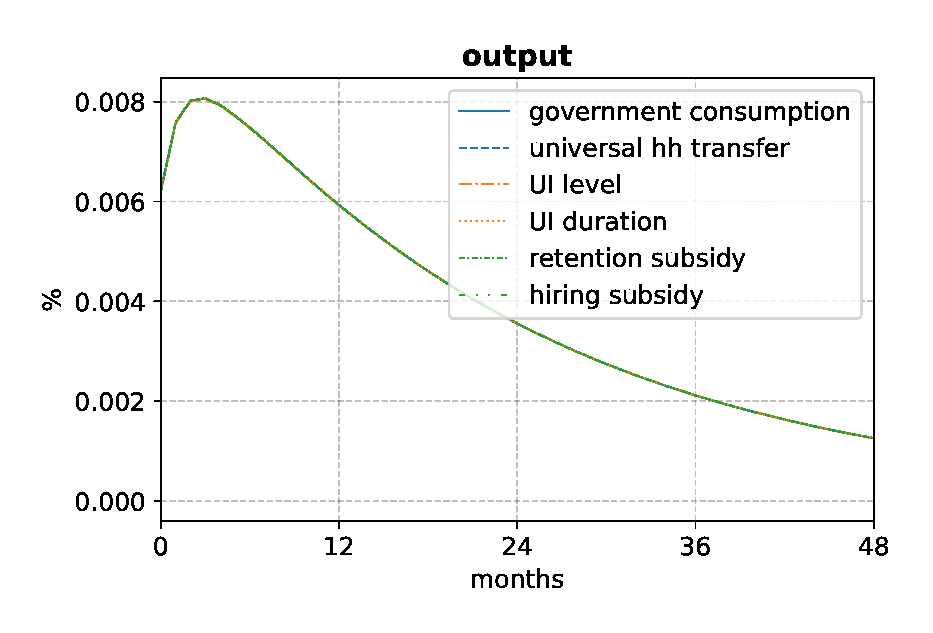
\includegraphics[width=0.45\linewidth]{results/policies_Y_titled} &  & 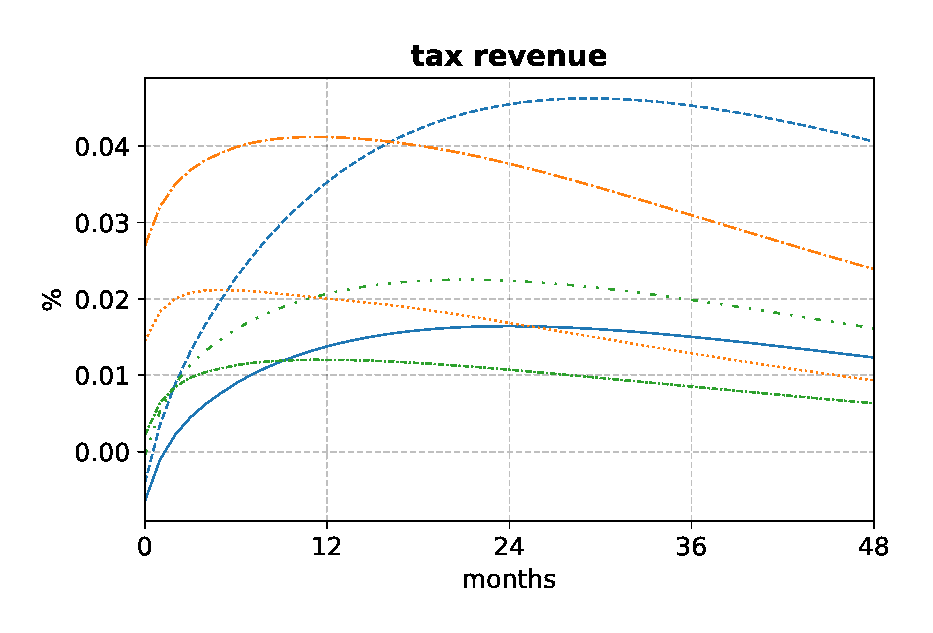
\includegraphics[width=0.45\linewidth]{results/policies_tax_titled}\tabularnewline
\end{tabular}
\begin{itemize}
\item Baseline policy: Persistent \textbf{G} shock ($\rho_{G}=0.965$).
\item Other policies chosen to yield identical output paths
\item Yet, starkly different paths of tax revenues $\Rightarrow$ different multipliers
\end{itemize}
\end{frame}

\begin{frame}{Fiscal multipliers relative to \textbf{G}}

\begin{table}
	\begin{center}
		\begin{tabular}{lcccccc}
\toprule
& &  \multicolumn{3}{c}{\hrulefill\,\,\textbf{HH transfers}\,\,\hrulefill} & \multicolumn{2}{c}{\hrulefill\,\,\textbf{Firm subsidies}\,\,\hrulefill} \\
& \textbf{G} [level] & \textbf{Transfer} & \textbf{Level} & \textbf{Duration} & \textbf{Retain} & \textbf{Hire} \\
\midrule
& 1.0 [0.99] & 0.28 & 0.44 & 1.03 & 1.64 & 0.72 \\
\bottomrule
\end{tabular}
  
	\end{center}
	\vspace{-2mm}
\end{table}
\vspace{1cm}
\begin{itemize}
	\item Fiscal Multiplier $= \frac{\sum output_t}{\sum spending_t}$
	
	\item Strong dispersion in multipliers.
	\item Retention subsidies most, universal transfers least stimulative
\end{itemize}
\end{frame}


\begin{frame}{Determinants of fiscal multipliers}
\vspace{1cm}
\begin{itemize}
	\item Identify determinants by reducing frictions one-by-one
\end{itemize}
\end{frame}
%
\begin{frame}{Determinants of fiscal multipliers}

\centering
\begin{small}
\setlength\tabcolsep{1.5pt} 
\begin{tabular}{lcccccc}
\toprule
& &  \multicolumn{3}{c}{\hrulefill\,\,\textbf{Household transfers}\,\,\hrulefill} & \multicolumn{2}{c}{\hrulefill\,\,\textbf{Firm transfers}\,\,\hrulefill} \\
& \textbf{G} [level] & \textbf{Transfer} & \textbf{Level} & \textbf{Duration} & \textbf{Retain} & \textbf{Hire} \\
\midrule
1. Baseline & 1.0 [0.99] & 0.28 & 0.44 & 1.03 & 1.64 & 0.72 \\
\midrule
2. Less sticky $P$ ($\phi \!=\! 178$) &&&&&&\\
3. Reactive mp ($\delta_\pi \!=\! 2$)  &&&&&&\\
\midrule
4. Representative agent &&&&&& \\
5. Fewer HtM (17.4\%)   &&&&&&\\
6. Reactive tax ($\omega \!=\! 0.10$) &&&&&& \\
\midrule
7. Ex. separations ($\psi \!=\! 0$)  &&&&&&\\
8. Free entry ($\xi \!=\! \infty$)  &&&&&& \\
9. Wage rule ($\eta_e \!=\! 0.50$)   &&&&&&\\
10. 95\% of div. to PIH   &&&&&&\\
\bottomrule
\end{tabular}
  
\end{small}
\vspace{-2mm}
\end{frame}
%
\begin{frame}{Benchmark $\boldsymbol{G}$ multiplier}

\centering
\begin{small}
\setlength\tabcolsep{1.5pt} 
\input{results/fiscal_multipliers_all_pres_G_1.tex}  
\end{small}

\begin{itemize}
\item Government-consumption multipliers increase with ...
\begin{itemize}
\item Nominal rigidity, passive MP, debt-financing, less-Ricardian HHs (Auclert
et al 2024, Hagedorn et al 2023) 
\end{itemize}
\end{itemize}
\end{frame}
%
\begin{frame}{Benchmark $\boldsymbol{G}$ multiplier}

\centering
\begin{small}
\setlength\tabcolsep{2.5pt} 
\begin{tabular}{lcccccc}
\toprule
& &  \multicolumn{3}{c}{\hrulefill\,\,\textbf{Household transfers}\,\,\hrulefill} & \multicolumn{2}{c}{\hrulefill\,\,\textbf{Firm transfers}\,\,\hrulefill} \\
& \textbf{G} [level] & \textbf{Transfer} & \textbf{Level} & \textbf{Duration} & \textbf{Retain} & \textbf{Hire} \\
\midrule
1. Baseline & 1.0 [\color{red}{\textbf{0.99}}] & 0.28 & 0.44 & 1.03 & 1.64 & 0.72 \\
\midrule
2. Less sticky $P$ ($\phi \!=\! 178$) & 1.0 [\color{red}{\textbf{0.61}}] &&&&& \\
3. Reactive mp ($\delta_\pi \!=\! 2$) & 1.0 [\color{red}{\textbf{0.64}}]  &&&&&\\
\midrule
4. Representative agent & 1.0 [\color{red}{\textbf{0.54}}] &&&&& \\
5. Fewer HtM (17.4\%) & 1.0 [\color{red}{\textbf{0.80}}] &&&&& \\
6. Reactive tax ($\omega \!=\! 0.10$) & 1.0 [\color{red}{\textbf{0.84}}]&&&&&  \\
\midrule
7. Ex. separations ($\psi \!=\! 0$) & 1.0 [\color{red}{\textbf{0.13}}] &&&&& \\
8. Free entry ($\xi \!=\! \infty$) & 1.0 [\color{red}{\textbf{0.54}}]  &&&&&\\
9. Wage rule ($\eta_e \!=\! 0.50$) & 1.0 [\color{red}{\textbf{0.73}}]  &&&&&\\
10. 95\% of div. to PIH & 1.0 [\color{red}{\textbf{0.82}}] &&&&& \\
\bottomrule
\end{tabular}
  
\end{small}
\begin{itemize}
\item Government-consumption multiplier increases with ...
\begin{itemize}
\item Nominal rigidity, passive MP, debt-financing, less-Ricardian HHs
\item SAM frictions, wage rigidity, MPC o/o profits
\end{itemize}
\end{itemize}
\end{frame}
%
\begin{frame}{Relative HH-transfer multipliers: non-HA frictions}

\centering
\begin{small}
\setlength\tabcolsep{2.5pt} 
\begin{tabular}{lcccccc}
\toprule
& &  \multicolumn{3}{c}{\hrulefill\,\,\textbf{Household transfers}\,\,\hrulefill} & \multicolumn{2}{c}{\hrulefill\,\,\textbf{Firm transfers}\,\,\hrulefill} \\
& \textbf{G} [level] & \textbf{Transfer} & \textbf{Level} & \textbf{Duration} & \textbf{Retain} & \textbf{Hire} \\
\midrule
1. Baseline & 1.0 [0.99] &  \color{red}{\textbf{0.28}} &  \color{red}{\textbf{0.44}} &  \color{red}{\textbf{1.03}} & & \\
\midrule
2. Less sticky $P$ ($\phi \!=\! 178$) & 1.0 [0.61] & \color{red}{\textbf{0.30}} & \color{red}{\textbf{0.47}} & \color{red}{\textbf{1.03}} & & \\
3. Reactive mp ($\delta_\pi \!=\! 2$) & 1.0 [0.64] & \color{red}{\textbf{0.30}} & \color{red}{\textbf{0.47}} & \color{red}{\textbf{1.03}} & & \\
\midrule
4. Representative agent & 1.0 [0.54] & 0.00 & 0.00 & 0.00 && \\
5. Fewer HtM (17.4\%) & 1.0 [0.80] & 0.19 & 0.41 & 1.11 & & \\
6. Reactive tax ($\omega \!=\! 0.10$) & 1.0 [0.84] & 0.19 & 0.40 & 1.10 & & \\
\midrule
7. Ex. separations ($\psi \!=\! 0$) & 1.0 [0.13] & \color{red}{\textbf{0.35}} & \color{red}{\textbf{0.52}} & \color{red}{\textbf{1.02}} & & \\
8. Free entry ($\xi \!=\! \infty$) & 1.0 [0.54] & \color{red}{\textbf{0.31}} & \color{red}{\textbf{0.47}} & \color{red}{\textbf{1.03}} & &\\
9. Wage rule ($\eta_e \!=\! 0.50$) & 1.0 [0.73] & \color{red}{\textbf{0.29}} & \color{red}{\textbf{0.46}} & \color{red}{\textbf{1.03}} & & \\
10. 95\% of div. to PIH & 1.0 [0.82] & \color{red}{\textbf{0.28}} & \color{red}{\textbf{0.43}} & \color{red}{\textbf{0.99}} & & \\
\bottomrule
\end{tabular}
  
\end{small}
\begin{itemize}
\item Relative HH transfer multipliers $\approx$ unaffected by non-HA frictions
\end{itemize}
\end{frame}
%
\begin{frame}{Relative HH-transfer multipliers: HA frictions}

\centering
\begin{small}
\setlength\tabcolsep{2.5pt} 
\begin{tabular}{lcccccc}
\toprule
& &  \multicolumn{3}{c}{\hrulefill\,\,\textbf{Household transfers}\,\,\hrulefill} & \multicolumn{2}{c}{\hrulefill\,\,\textbf{Firm transfers}\,\,\hrulefill} \\
& \textbf{G} [level] & \textbf{Transfer} & \textbf{Level} & \textbf{Duration} & \textbf{Retain} & \textbf{Hire} \\
\midrule
1. Baseline & 1.0 [0.99] & 0.28 & 0.44 & 1.03 & 1.64 & 0.72 \\
\midrule
2. Less sticky $P$ ($\phi \!=\! 178$) & 1.0 [0.61] & 0.30 & 0.47 & 1.03 & & \\
3. Reactive mp ($\delta_\pi \!=\! 2$) & 1.0 [0.64] & 0.30 & 0.47 & 1.03 & &\\
\midrule
4. Representative agent & 1.0 [0.54] & \color{red}{\textbf{0.00}} & \color{red}{\textbf{0.00}} & \color{red}{\textbf{0.00}} && \\
5. Fewer HtM (17.4\%) & 1.0 [0.80] & \color{red}{\textbf{0.19}} & \color{red}{\textbf{0.41}} & \color{red}{\textbf{1.11}} & 1& \\
6. Reactive tax ($\omega \!=\! 0.10$) & 1.0 [0.84] & \color{red}{\textbf{0.19}} & \color{red}{\textbf{0.40}} & \color{red}{\textbf{1.10}} & & \\
\midrule
7. Ex. separations ($\psi \!=\! 0$) & 1.0 [0.13] & 0.35 & 0.52 & 1.02 && \\
8. Free entry ($\xi \!=\! \infty$) & 1.0 [0.54] & 0.31 & 0.47 & 1.03 && \\
9. Wage rule ($\eta_e \!=\! 0.50$) & 1.0 [0.73] & 0.29 & 0.46 & 1.03 & & \\
10. 95\% of div. to PIH & 1.0 [0.82] & 0.28 & 0.43 & 0.99 & & \\
\bottomrule
\end{tabular}
  
\end{small}
\begin{itemize}
\item Ricardian households: zero transfer multipliers
\item Lower MPC lowers transfer multipliers \& \uline{raises} duration multiplier
\item Same holds for more tax financing
\end{itemize}
\end{frame}
%
\begin{frame}{Relative firm-subsidy multipliers: non-SAM frictions}

\centering
\begin{small}
\setlength\tabcolsep{2.5pt} 
\input{results/fiscal_multipliers_all_pres_S.tex}  
\end{small}

\begin{itemize}
\item Relative multipliers of subsidies $\approx$ unaffected by non-SAM
frictions
\item Less nominal rigidity: subsidies more effective wrt HH transfers/$G$
\end{itemize}
\end{frame}
%
\begin{frame}{Relative firm-subsidy multipliers: SAM frictions}

\centering
\begin{small}
\setlength\tabcolsep{2.5pt} 
\input{results/fiscal_multipliers_all_pres_S_SAM.tex}  
\end{small}

\begin{itemize}
\item {\small Hiring subsidy more effective with higher entry/lower separation
elasticity}{\small\par}
\item Lower MPC o/o profits weakens both subsidies
\end{itemize}
\end{frame}


%\begin{frame}
%
%\begin{center}
%	\huge Q\&A Session \normalfont
%\end{center}
%
%\end{frame}
%
%
%\begin{frame}{Questions}
%\begin{itemize}
%	\setlength\itemsep{1em}	
%	
%	\item Exam 2023 May Question 2: First sub question: Could you explain a bit more how we should arrive at this conclusion from the solutions: ``Given that the shock occurs in the Firm optimality condition (3), lets take as given that inflation growth  declines.? This of course sounds reasonable to assume but I am a bit confused what to assume and how to proceed. If we did not start by this assumption, can we still arrive at the right description of what happens in the problem?''
%	
%	\item Lecture 9: slide 36: Could you show how to arrive at the wage curve when we have endogenous separation? 
%	
%	\item How should one think when stating a social planner problem? It is not clear which components to include
%	
%	\item  If you have found the optimal conditions for, for example, households and companies. Why should you stop at restrictions and other conditions to find the solution in general equilibrium. This is done, among other things, in growth models, and in the Aiygari model?
%	
%	\item How should one think when starting to solve a specific problem. Which equations to include, and which to not include?
%	
%\end{itemize}
%\end{frame}
%
%\begin{frame}{Questions}
%\begin{itemize}
%	\setlength\itemsep{1em}	
%	
%	\item I am a bit confused by the Rothschild critique and the Diamond paradox in the McCall model. I think we have already discussed this, but I am still confused: why firms do not offer an epsilon above the wage set by all other firms? In the Burdett-Mortensen this is the reason for which we don?t have a degenerate wage distribution, but why it is not the case here?
%	
%	\item In the Burdett-Mortensen, the support of the wage distribution is $[w_R, y]$. But given that the profit is equal for every wage in the support, this means that every firm is making zero profits (because at least one firm will offer exactly y). Is that the case? Also, does the wage distribution imply that every wage has a positive probability of being offered (i.e., there is at least one firm offering a wage in the support) or that every firm is offering every wage with positive probability? I read somewhere that they were saying``equilibrium has to be a mixed-strategy equilibriu'', and this to me sounds like the latter hypothesis.
%	
%	\item DMP: Statics, slide 21/43: ?Given theta, we can solve for {v,u}?, what does it mean? Because it seems to me that we end up with theta=v/u, but this we already knew from the definition of theta.
%	
%	\item Incomplete markets: basics, slide 32/42: if credit constraint binds, MPC is high. Why is that? Is it because this implies that the marginal utility of consumption today is higher than the expected marginal value of assets tomorrow $V_m(M?)$?
%	
%\end{itemize}
%\end{frame}
%
%
%\begin{frame}{Questions}
%\begin{itemize}
%	\setlength\itemsep{1em}	
%	
%	\item Exam 2023 May Question 2: First sub question: Could you explain a bit more how we should arrive at this conclusion from the solutions: ``Given that the shock occurs in the Firm optimality condition (3), lets take as given that inflation growth  declines.? This of course sounds reasonable to assume but I am a bit confused what to assume and how to proceed. If we did not start by this assumption, can we still arrive at the right description of what happens in the problem?''
%	
%\end{itemize}
%\end{frame}
%
%
%\begin{frame}{Exam 2023 May Question 2}
%\begin{itemize}
%	\setlength\itemsep{1em}	
%	
%	\item Question: Explain the sign of all responses for all variables displayed in Figure 1.
%	
%	\item Equilibrium system
%	\begin{eqnarray*}
%	\text{Intratemporal hh optimality:} && \hat \omega_t = \hat c_t + \varphi \hat n_t   \\
%	\text{Intertemporal hh optimality:} && \hat c_t =  - (\hat i_t - E_t \pi_{t+1}) + E_t \hat c_{t+1}  \\
%	\text{Firm optimality:} && \pi_t = \beta E_t \pi_{t+1} + \lambda \widehat{mc}_t + \nu_t  \\
%	\text{Marginal cost:} && \widehat{mc}_t = \hat \omega_t  \\
%	\text{Goods clearing:} && \hat c_t = \hat y_t \\
%	\text{Labor clearing:} && \hat y_t = \hat n_t  \\
%	\text{Policy:} && \hat i_t = \phi \pi_t 
%	\end{eqnarray*}
%	
%\end{itemize}
%\end{frame}
%
%\begin{frame}{Exam 2023 May Question 2:}
%
%\begin{figure}
%	\centering
%	\includegraphics[scale=0.5,trim= 0 200 0 200, clip]{figures/nk_cpshock_9variables.pdf}
%	\caption{IRFs to a cost push shock in the vanilla NK model}
%\end{figure}
%
%\end{frame}
%
%\begin{frame}{Exam 2023 May Question 2:}
%
%\begin{itemize}
%	\setlength\itemsep{1em}	
%	
%	\item General approach to questions like this: ``Guess and verify'' 
%	
%	\item You can start in many places, my suggested solution starts in Firm optimality condition
%	\begin{eqnarray*}
%		\pi_t = \beta E_t \pi_{t+1} + \lambda \widehat{mc}_t + \nu_t  
%	\end{eqnarray*}
%or
%	\begin{eqnarray*}
%	- \left(\beta E_t \pi_{t+1} -\pi_t  \right)=  \lambda \widehat{mc}_t + \nu_t  
%\end{eqnarray*}
%
%	\item My reasoning:
%	\bit
%		\item Firm optimality: holding $\hat mc_t$ constant, positive shock depresses inflation growth $\beta E_t \pi_{t+1}-\pi_t<0$. So lets assume $\beta E_t \pi_{t+1}-\pi_t<0$
%
%		\item Unique bounded equilibrium  $\Rightarrow$ inflation $\pi_t>0$ 
%
%		\item Policy rule + intertemporal optimality $\Rightarrow$ $c_t<0$
%
%		\item Intratemporal optimality + market clearing $mc_t <0$
%	\eit
%	
%	\item Suppose we would instead have assumed that $\beta E_t \pi_{t+1}-\pi_t>0$ constant. 
%	\bit
%		\item Then, following the same steps, we would have concluded $mc_t>0$.	
%		
%		\item Then we get a contradiction in the firm optimality condition
%	\eit
%		
%\end{itemize}
%\end{frame}
%
%
%\begin{frame}{Questions}
%\begin{itemize}
%	\setlength\itemsep{1em}	
%	
%	
%	\item  \color{black} Lecture 9: slide 36: Could you show how to arrive at the wage curve when we have endogenous separation? 
%	
%\end{itemize}
%\end{frame}
%
%\begin{frame}{Lecture 9: Equilibrium definition (Typo in lecture notes!!)}
%
%\bit
%\setlength\itemsep{1em}
%
%\item An equilibrium is a collection $\{W,U, J, V, w, x_R, \theta\}$ s.t. the following equations hold
%\bit
%\item \bf Bellman equations:
%\begin{eqnarray}
%rW(x) &=& w(x)  + \lambda_x \left[ \int_{x_R}^{1} (W(x')-W(x)) d\Gamma (x') - (U-W(x))\Gamma (x_R)  \right] \nonumber \\ 
%rU &=& b  + \lambda_u(\theta) \left(W(1)-U\right) \nonumber \\
%rJ(x) &=& xy - w(x)+\lambda_x \left[ \int_{x_R}^{1} (J(x')-J(x)) d\Gamma (x') - (V-J(x))\Gamma (x_R)  \right] \nonumber \\
%rV &=& -c +\lambda_v(\theta)\left(J(1)-V\right) \nonumber
%\end{eqnarray}
%
%\item Separation decision:
%\begin{eqnarray}
%J(x_R) &=& V \nonumber 
%\end{eqnarray}
%
%\item Free entry:
%\begin{eqnarray}
%V &=& 0 \nonumber 
%\end{eqnarray}
%
%\item Wage setting rule: \normalfont
%\begin{eqnarray}
%\gamma (J(x)-V) = (1-\gamma) (W(x)-U) \nonumber
%\end{eqnarray}
%\eit
%
%\item 7 equations, 7 unknowns
%\eit
%\end{frame}
%
%\begin{frame}{Lecture 9: Equilibrium definition (corrected)}
%
%\bit
%\setlength\itemsep{1em}
%
%\item An equilibrium is a collection $\{W,U, J, V, w, x_R, \theta\}$ s.t. the following equations hold
%\bit
%\item \bf Bellman equations:
%\begin{eqnarray}
%rW(x) &=& w(x)  + \lambda_x \left[ \int_{x_R}^{1} (W(x')-W(x)) d\Gamma (x') + (U-W(x))\Gamma (x_R)  \right] \nonumber \\ 
%rU &=& b  + \lambda_u(\theta) \left(W(1)-U\right) \nonumber \\
%rJ(x) &=& xy - w(x)+\lambda_x \left[ \int_{x_R}^{1} (J(x')-J(x)) d\Gamma (x') + (V-J(x))\Gamma (x_R)  \right] \nonumber \\
%rV &=& -c +\lambda_v(\theta)\left(J(1)-V\right) \nonumber
%\end{eqnarray}
%
%\item Separation decision:
%\begin{eqnarray}
%J(x_R) &=& V \nonumber 
%\end{eqnarray}
%
%\item Free entry:
%\begin{eqnarray}
%V &=& 0 \nonumber 
%\end{eqnarray}
%
%\item Wage setting rule: \normalfont
%\begin{eqnarray}
%\gamma (J(x)-V) = (1-\gamma) (W(x)-U) \nonumber
%\end{eqnarray}
%\eit
%
%\item 7 equations, 7 unknowns
%\eit
%\end{frame}
%
%\begin{frame}{Questions}
%\begin{itemize}
%	\setlength\itemsep{1em}	
%
%	
%	\item \color{black} How should one think when stating a social planner problem? It is not clear which components to include
%	
%\end{itemize}
%\end{frame}
%
%\begin{frame}{Social planners problem}
%\begin{itemize}
%	\setlength\itemsep{1em}	
%	
%	\item For any model, the unconstrained social planner optimize ``social welfare'' taking ``technological constraints'' as given
%	\bit
%		\item Typically, social welfare $=$ Utilitarian welfare
%		
%		\item ``Technological constraints'' = Resource constraint, production technology
%		
%		\item Importantly, the planner does not need to respect individual budgets nor prices
%	\eit
%	
%	\item Planner's problem in the RBC model:
%	\begin{eqnarray}
%	\max_{C_t, K_{t+1}, N_{t}} && \sum_{t=0}^{\infty} \beta^t \left[U(C_t)-V(N_t)\right] \nonumber \\
%	\text{s.t.} && C_t + (K_{t+1}-(1-\delta)K_t) = F(K_t, N_t) \nonumber
%	\end{eqnarray}
%	
%	
%	\item (Static) Planner's problem in the NK model:
%	\begin{eqnarray}
%	\max_{C_t, N_{it}} && \log C_t - \theta \frac{N_t^{1+\varphi}}{1+\varphi} \nonumber \\
%	\text{s.t.} && C_t = \left(\int_{0}^{1} (A_t N_{it})^{\frac{\epsilon-1}{\epsilon}} di \right)^{\frac{\epsilon}{\epsilon-1}} \nonumber \\
%	&& N_t = \int_{0}^{1} N_{it} di \nonumber
%	\end{eqnarray}
%	
%\end{itemize}
%\end{frame}
%
%
%\begin{frame}{Constrained Social planners problem}
%\begin{itemize}
%	\setlength\itemsep{1em}	
%	
%	\item A constrained social planner typically refers to a planner that can set the decisions of all agents, but need to respect the constraints each agent face
%
%	
%	\item Constrained planner's problem in the DMP model
%	\begin{eqnarray}
%	\max_{v} && \int_{0}^{\infty} e^{-rt}\left((1-u)y + ub- v c \right) dt \nonumber \\
%	\text{s.t.} &&  \dot{u} = \sigma (1-u) - \lambda_u(\frac{v}{u})u \nonumber 
%	\end{eqnarray}
%	
%	\item Unconstrained planner's problem in the DMP model
%	\begin{eqnarray}
%	\max_{u, v} && \int_{0}^{\infty} e^{-rt}\left((1-u)y + ub- v c \right) dt \nonumber 
%	\end{eqnarray}
%	
%\end{itemize}
%\end{frame}
%
%\begin{frame}{Questions}
%\begin{itemize}
%	\setlength\itemsep{1em}	
%	
%	\item  \color{black} If you have found the optimal conditions for, for example, households and companies. Why should you stop at restrictions and other conditions to find the solution in general equilibrium. This is done, among other things, in growth models, and in the Aiygari model?
%	
%\end{itemize}
%\end{frame}
%
%
%\begin{frame}{When to use which equation and where?}
%\begin{itemize}
%	\setlength\itemsep{1em}	
%	
%	\item In general, ``solving'' a model amounts to express endogenous variables as functions of exogenous parameters
%	
%	\item In an equilibrium model, what constitutes a ``solution'' is given by your equilibrium definition!
%	
%	\item If this can be done analytically, we get a closed-form expression for that function
%	
%	\item If not, we can off characterize the model anlytically (N equations in N unknowns), as we do with the RBC or the NK model
%	
%	\item Sometimes, we can extract properties about the model behavior without fully solving it
%	
%	\bit
%		\item Example: the equation for wage dispersion in McCall:
%		\begin{eqnarray}
%		Mm = \frac{\bar w}{w_R} = \frac{\frac{\lambda}{r+\sigma}+1}{\frac{\lambda}{r+\sigma}+\rho \nonumber}
%		\end{eqnarray} 
%	\eit  
%	
%	\item When it comes to answering questions on the exam, go as far as you need in terms of ``solving'' model in order to adequatly answer the question
%	
%\end{itemize}
%\end{frame}
%
%\begin{frame}{Example: May 2023: Question 3.2 (put exam on screen)}
%\begin{itemize}
%	\setlength\itemsep{1em}	
%	
%	\item To solve for the equilibrium level of interest rate, we need to solve for the crossing of asset demand and asset supply
%	
%	\item Solve for one household $=$ combine optimality condition with budget constraint
%	
%	\item Sum over all households to get total asset supply
%	
%	\item Asset demand come from Firm F.O.C.
%	
%	\item Equate asset demand with asset supply by inserting Firm F.O.C. in asset supply equation
%	
%\end{itemize}
%\end{frame}
%
%
%\begin{frame}{Questions}
%\begin{itemize}
%	\setlength\itemsep{1em}	
%	
%	\item \color{black} How should one think when starting to solve a specific problem. Which equations to include, and which to not include?
%	
%\end{itemize}
%\end{frame}
%
%
%\begin{frame}{How to approach a problem}
%\begin{itemize}
%	\setlength\itemsep{1em}	
%	
%	\item Answer is always context specific
%	
%	\item In terms of grading your answer, I look for whether you have demonstrated that you have understood the solution. Sometimes this requires stating the whole model, sometimes you can jump directly to an equilibrium condition
%	
%	\item I expect you to be able to state all the equations/assumptions of the models we have covered in class, but....
%	
%	\item ... many questions can be answered without stating all the assumptions of the model
%	
%	\item Some advice:
%	\bit
%		\setlength\itemsep{0.5em}
%		\item In general, whenever you are not sure, state more rather than less assumptions/equations 
%		
%		\item Search for symmetries: Is there a way to recast to problem so that it looks like a problem we've previously looked at
%		
%		\item Don't let algebraic mistakes stop you. If you some intution about how to get to the solution, write it out even if the equations are failing you
%	\eit
%	
%\end{itemize}
%\end{frame}
%
%
%\begin{frame}{Questions}
%\begin{itemize}
%	\setlength\itemsep{1em}	
%	
%	\item I am a bit confused by the Rothschild critique and the Diamond paradox in the McCall model. I think we have already discussed this, but I am still confused: why firms do not offer an epsilon above the wage set by all other firms? In the Burdett-Mortensen this is the reason for which we don?t have a degenerate wage distribution, but why it is not the case here?
%	
%\end{itemize}
%\end{frame}
%
%\begin{frame}{The McCall model}
%
%\bit
%\setlength\itemsep{1.5em}
%
%\item In the basic McCall model, all workers have the same reservation wage
%
%\item When there is only one reservation wage, this implies that if you, as a firm, offer $x+\epsilon$, when all other firms offer $x>w_{R}$, will not attract more workers
%
%\item Neither will you attract fewer workers in you post $x-\epsilon$
%
%\item Optimal wage posting strategy in such an environment just amounts to posting $w_{R}$
%
%\item In Burdett-Mortensen, workers have different reservation wages, due to the fact they have different wages, and search while employed
%
%\item Here, you can potentially attract more workers (by getting more acceptances), if you raise the wage
%
%\eit
%\end{frame}
%
%
%\begin{frame}{Questions}
%\begin{itemize}
%	\setlength\itemsep{1em}	
%	
%	\item In the Burdett-Mortensen, the support of the wage distribution is $[w_R, y]$. But given that the profit is equal for every wage in the support, this means that every firm is making zero profits (because at least one firm will offer exactly y). Is that the case? Also, does the wage distribution imply that every wage has a positive probability of being offered (i.e., there is at least one firm offering a wage in the support) or that every firm is offering every wage with positive probability? I read somewhere that they were saying``equilibrium has to be a mixed-strategy equilibriu'', and this to me sounds like the latter hypothesis.
%	
%\end{itemize}
%\end{frame}
%
%
%\begin{frame}{Equilibrium definition in Burdett-Mortensen}
%
%\bit
%\setlength\itemsep{1.5em}
%
%\item An equilibrium is a collection $\{w_R, \pi, F, \mathbb{W}_F\}$ such that
%\ben
%\setlength\itemsep{1em}
%\item Given $F$, each worker behaves optimally: $w_R$ solves reservation wage equation \eqref{reservation_wage_final} 
%
%\item Given $F$ and $w_R$, each firm behaves optimally:  $\pi$ follows from \eqref{firm_problem}
%
%\item $F, \mathbb{W}_F$ are such that there is no arbitrage:
%\begin{eqnarray}
%(y-w)I(w) \left\{ \begin{array}{cc}
%< \pi & \text{if } w \notin \mathbb{W}_F \\
%= \pi & \text{if } w \in \mathbb{W}_F
%\end{array} \right. \nonumber
%\end{eqnarray}
%where $\mathbb{W}_F$ is the support of $F$
%\een
%
%\eit
%
%\end{frame}
%
%\begin{frame}{Comments}
%
%\bit
%\setlength\itemsep{1.5em}
%
%\item >Expected profits< are equilized in equilibrium, not actual profits
%
%\item The equilibrium is solved for in 5 steps
%
%\item Step 1: $\mathbb{W}_F =[w_{min}, w_{max}] \in [w_R, y]$
%
%\item Step 4: $w_{max} < y$
%
%\item Positive expected profits in equilibrium!
%
%\item We solved for a pure-strategy equilibrium, but mixed strategy also works!
%
%\eit
%
%\end{frame}
%
%
%\begin{frame}{Step 1: bounded support}
%
%\bit
%\setlength\itemsep{2em}
%
%\item No worker accept a wage $w< w_R \Rightarrow$ $\pi(w<w_R) = 0$
%
%\item Also, $\pi(w>y) < 0$
%
%\item Ergo, F has bounded support $[\underbar w, \bar w] \subset [w_R, y]$
%
%\eit
%
%\end{frame}
%
%\begin{frame}{Step 2: continuity}
%
%\bit
%\setlength\itemsep{1em}
%
%\item Proof strategy: If $F$ has a mass point $\hat w$, you make excess profits by offering $\hat w + \epsilon$
%
%\item Assume $F$ has a mass point at $\hat w$: {\rc (Draw graph on whiteboard)}
%\begin{eqnarray}
%F(\hat w) = F(\hat w^{-}) + v_1(\hat w) \text{  where $v_1(\hat w)>0$ }\nonumber
%\end{eqnarray}
%
%\item Then, average firm size $I$ is discontinuous at $\hat w$: {\rc (Do on whiteboard)}
%\begin{eqnarray}
%I(\hat w^{+}) = I(\hat w) + v_2(\hat w) \text{  where $v_2(\hat w)>0$ } \nonumber
%\end{eqnarray}
%
%\item Then,
%\begin{eqnarray}
%\lim\limits_{\epsilon \rightarrow 0} \pi(\hat w+\epsilon)-\pi(\hat w) &=& \lim\limits_{\epsilon \rightarrow 0} (y-\hat w-\epsilon) I(\hat{w}+\epsilon) - (y-\hat w) I(\hat{w}) \nonumber \\
%&=& \lim\limits_{\epsilon \rightarrow 0} (y-\hat w)(I(\hat{w}+\epsilon)-I(\hat{w})) -\epsilon I(\hat{w}+\epsilon) \nonumber \\
%&=& \lim\limits_{\epsilon \rightarrow 0}  (y-\hat w)(I(\hat{w}+\epsilon)-I(\hat{w})) \nonumber \\ 
%&=& (y-\hat w)v_2(\hat w)  \nonumber \\ 
%&>& 0 \nonumber 
%\end{eqnarray}
%
%\item You can make excess profits by offering wage contract $\hat{w}+\epsilon$ because
%\bit
%\item per worker profit decrease continuously
%\item firm competition decrease discretely 
%\eit
%
%\eit
%
%\end{frame}
%
%
%
%\begin{frame}{Step 3: $\underbar w = w_R$}
%
%\bit
%\setlength\itemsep{1em}
%
%\item Step 1: $\mathbb{W}_F =[\underbar w, \bar w] \subset [w_R, y]$ 
%
%\item Step 2: $F$ is continuous:
%\begin{eqnarray}
%I(w) &=&  \frac{k_u (1+k_e(1-F(W_R)))/(1+k_u(1-F(w_R)))}{(1+k_e(1-F(w)))(1+k_1(1-F(w^{-})))} \nonumber \\
%&=&  \frac{k_u (1+k_e(1-F(w_R)))/(1+k_u(1-F(w_R)))}{(1+k_e(1-F(w)))^2} \nonumber
%\end{eqnarray}
%for $w \geq w_R$. 
%
%\item Moreover $F(\underbar w) = 0$, which in turn implies $F(w_R)=0$
%
%\item Hence, 
%\begin{eqnarray}
%I(\underbar w) =  \frac{k_u (1+k_e)/(1+k_u)}{(1+k_e)^2} =  \frac{k_u /(1+k_u)}{(1+k_e)} \nonumber
%\end{eqnarray}
%
%\item Expected firm size at $\underbar w$ is independent of the particular value of $\underbar w$!
%
%\item Therefore, $\underbar w = w_R$, since if $\underbar w > w_R$, a firm could offer $w_R$ and get the same amount of workers and higher per worker profits $\Rightarrow$ excess profits
%%
%%\item Notice: $\pi=\pi(w_R)=(p-w_R)I(\underbar w)>0$. Why?
%
%\eit
%
%\end{frame}
%
%
%\begin{frame}{Step 4: solve for F}
%
%\bit
%\setlength\itemsep{1.5em}
%
%\item In equilibrium, $\pi(w) = \pi(w')$ for all $w, w' \in \mathbb{W}_F$
%
%\item In particular, $\pi(w) = \pi(w_R)$ for all $w \in \mathbb{W}_F$
%
%\item Solve $\pi(w) = \pi(w_R)$, using our solutions for $I(w), I(w_R)$:
%\begin{eqnarray}
%(y-w)I(w) &=& (y-w_R)I(w_R) \Leftrightarrow \nonumber \\
%(y-w)\frac{k_u (1+k_e)/(1+k_u)}{(1+k_e(1-F(w)))^2} &=& (y-w_R) \frac{k_u /(1+k_u)}{(1+k_e)} \nonumber
%\end{eqnarray}
%\item Do the algebra to find
%\begin{eqnarray}
%F(w) = \frac{1+k_e}{k_e} \left[1-\left(\frac{y-w}{y-w_R}\right)^{1/2}\right]
%\end{eqnarray}
%
%\item Using that $F(\bar w) = 1$, we see that $\bar w<y$:
%\begin{eqnarray}
%\bar w = y - \frac{y-w_R}{(1+k_e)^2}<y
%\end{eqnarray}
%
%\eit
%
%\end{frame}
%
%
%\begin{frame}{Step 5: solve for $w_R$}
%
%\bit
%\setlength\itemsep{1.5em}
%
%\item Our reservation wage equation \eqref{reservation_wage_final}:
%\begin{eqnarray}
%w_R-b = (\lambda_u-\lambda_e) \int_{w \geq w_R}\frac{1-F(w)}{r+\sigma + \lambda_e(1-F(w))} dw \nonumber
%\end{eqnarray}
%\item For simplicity, we use the assumption $r \rightarrow 0$ again: 
%\begin{eqnarray}
%w_R-b = (k_u-k_e) \int_{w \geq w_R}\frac{1-F(w)}{1 + k_e(1-F(w))} dw \nonumber
%\end{eqnarray}
%\item Plug in the solution of $F$:
%%\begin{eqnarray}
%%w_R-b = \frac{(k_u-k_e)}{k_e} \int_{w_R}^{\bar w}\frac{k_e \left(\frac{y-w}{y-w_R}\right)^{1/2}-1}{k_e\left(\frac{y-w}{y-w_R}\right)^{1/2} + 1} dw \nonumber
%%\end{eqnarray}
%\begin{eqnarray}
%w_R-b = \frac{(k_u-k_e)}{k_e} \int_{w_R}^{\bar w} \left[1-\frac{1}{1+k_e} \left( \frac{y-w}{y-w_R}\right)^{-\frac{1}{2}}\right]dw \nonumber
%\end{eqnarray}
%\item Solve the integral and use the solution to $\bar w$ to find:
%\begin{eqnarray}
%w_R = \frac{(1+k_e)^2b + (k_u-k_e)k_ey}{(1+k_e)^2+(k_u-k_e)k_e}
%\end{eqnarray}
%
%\item Summary: a continuous offer distribution with $b<\underbar w = w_R< \bar w<y$!
%\eit
%
%
%\end{frame}
%
%
%
%\begin{frame}{Questions}
%\begin{itemize}
%	\setlength\itemsep{1em}	
%	
%	\item DMP: Statics, slide 21/43: ``Given theta, we can solve for {v,u}'', what does it mean? Because it seems to me that we end up with theta=v/u, but this we already knew from the definition of theta.
%	
%\end{itemize}
%\end{frame}
%
%
%\begin{frame}{Equilibrium definition in DMP}
%
%\bit
%\setlength\itemsep{1.5em}
%
%\item An equilibrium is a collection $\{W,U, J, V, w, \theta\}$ s.t. the following equations hold
%\bit
%\item \bf Bellman equations:
%\begin{eqnarray}
%rW &=& w  + \sigma \left(U-W \right) \nonumber \\ 
%rU &=& b  + \lambda_u(\theta) \left(W-U\right) \nonumber \\
%rJ &=& (y-w)  + \sigma \left(V-J\right) \nonumber \\ 
%rV &=& -c  + \lambda_v(\theta) \left(J-V\right) \nonumber
%\end{eqnarray}
%
%\item Free entry:
%\begin{eqnarray}
%V &=& 0 \nonumber 
%\end{eqnarray}
%
%\item Wage setting rule: \normalfont
%\begin{eqnarray}
%\gamma (J-V) = (1-\gamma) (W-U) \nonumber
%\end{eqnarray}
%\eit
%
%\item Six equations, six unknowns
%
%\item Given $\theta$, we can solve for $\{v,u\}$ from
%\begin{eqnarray}
%\dot{u} &=& \sigma (1-u) + \lambda_u(\theta)u \nonumber \\
%u(0) &=& \underbar{u} \nonumber \\
%\theta &=& \frac{v}{u} \nonumber
%\end{eqnarray}
%\eit
%\end{frame}
%
%
%\begin{frame}{DMP equilibrium: comment}
%\begin{itemize}
%	\setlength\itemsep{1em}	
%	
%	\item The six first equations solve for $\theta$
%	
%	\item Given $\theta$, we know $\lambda_u(\theta)$
%	
%	\item Then we know the transition rates  of the law-of-motion for unemployment
%	\begin{eqnarray}
%	\dot{u} &=& \sigma (1-u) + \lambda_u(\theta)u \nonumber 
%	\end{eqnarray}
%	
%	\item Together with some initial condition $u(0) = \underbar{u}$, we can solve for the path of unemployment $u_t$
%	
%	\item We solved for a steady state in $\theta$, but not in $u$!!
%	
%	\item Later, we showed that steady state $u=\frac{\sigma}{\sigma +\lambda_u(\theta)}$ is a very good approximation for $u_t$ given high transition rates 
%	
%\end{itemize}
%\end{frame}
%
%
%\begin{frame}{Questions}
%\begin{itemize}
%	\setlength\itemsep{1em}	
%	
%	\item Incomplete markets: basics, slide 32/42: if credit constraint binds, MPC is high. Why is that? Is it because this implies that the marginal utility of consumption today is higher than the expected marginal value of assets tomorrow $V_m(M?)$?
%	
%\end{itemize}
%\end{frame}
%
%
%\begin{frame}{Income-Fluctuations Problem}
%
%\bit
%\setlength\itemsep{2em}
%
%\item Recursive problem:
%\begin{eqnarray}
%V(M) &=& \max_{C, M'} U(C) + \beta E V(M') \nonumber \\
%\text{s.t.} && M' \leq R(M-C)+Y' \nonumber \\
%&& C \leq M \nonumber
%\end{eqnarray}
%
%\item We showed that global solution $C=C(M)$ therefore satisfies
%\begin{eqnarray}
%C(M) = \left\{ \begin{array}{cc}
%M & \text{if } M\leq M^* \\
%(U_c)^{-1}\left[ \beta R  E U_c(C') \right] &\text{if } M> M^*
%\end{array}\right. \nonumber
%\end{eqnarray}
%for some cutoff $M^*$
%
%\item When cc binds, we have $C(M) = M$, and $MPC = \frac{\partial C}{\partial M} = 1$
%
%\item When cc binds, we must have that $U_c(C) > \beta R  E U_c(C')$ (lack of consumption smoothing!)
%
%\eit
%
%\end{frame}
%



\end{document}



\begin{frame}{Questions}
\begin{itemize}
	\setlength\itemsep{1em}	
	
	\item I am a bit confused by the Rothschild critique and the Diamond paradox in the McCall model. I think we have already discussed this, but I am still confused: why firms do not offer an epsilon above the wage set by all other firms? In the Burdett-Mortensen this is the reason for which we don?t have a degenerate wage distribution, but why it is not the case here?
	
	\item In the Burdett-Mortensen, the support of the wage distribution is $[w_R, y]$. But given that the profit is equal for every wage in the support, this means that every firm is making zero profits (because at least one firm will offer exactly y). Is that the case? Also, does the wage distribution imply that every wage has a positive probability of being offered (i.e., there is at least one firm offering a wage in the support) or that every firm is offering every wage with positive probability? I read somewhere that they were saying``equilibrium has to be a mixed-strategy equilibriu'', and this to me sounds like the latter hypothesis.
	
	\item DMP: Statics, slide 21/43: ?Given theta, we can solve for {v,u}?, what does it mean? Because it seems to me that we end up with theta=v/u, but this we already knew from the definition of theta.
	
	\item Incomplete markets: basics, slide 32/42: if credit constraint binds, MPC is high. Why is that? Is it because this implies that the marginal utility of consumption today is higher than the expected marginal value of assets tomorrow $V_m(M?)$?
	
\end{itemize}
\end{frame}



